\section{Introducción a tipos sesión}

\begin{frame}{\insertsection}

	El desarrollo de software distribuido se enfoca principalmente en la
	integración, cooperación y comunicación de componentes en un sistema.

	\bigskip

	Dificultades:
	\begin{itemize}
		\item{Desafío tecnológico}
		\item{\alert<2>{Razonamiento sobre el sistema}}
		\pause
	\end{itemize}

	\note{Primero introducción a qué son y
	qué problema buscan resolver los tipos sesión. Después charlar sobre la
	variante probabilística. Luego el objetivo de este trabajo y un paseo
	por el mismo.}
	\note{Desafío tecnológico: trabajo correspondiente a la
	integración concreta de los componentes. Implementación.
	\\
	Razonamiento: comprender el estado de un sistema distribuido.}
\end{frame}

\begin{frame}{\insertsection}
	\begin{figure}
		\centering
		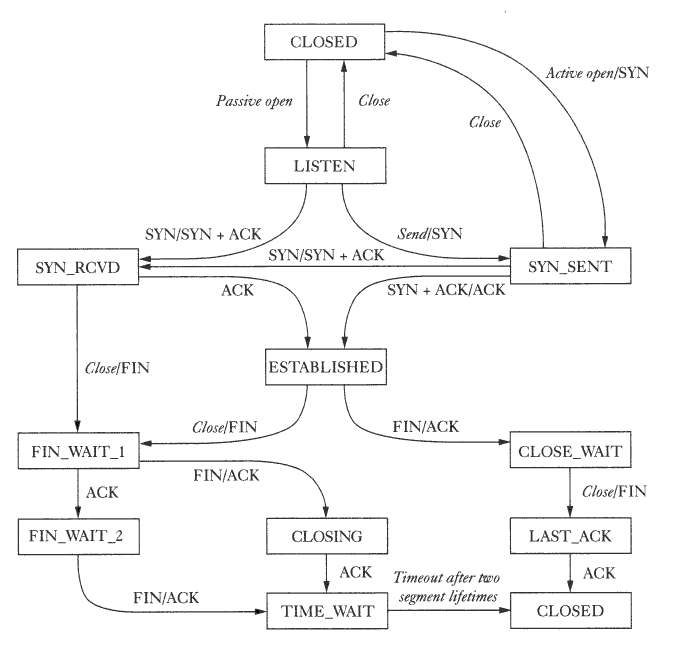
\includegraphics[width=0.6\textwidth]{images/tcp-state-diagram.png}
		\caption{Diagrama de estados para protocolo \textsc{TCP}}
	\end{figure}
	\note{Mostrar brevemente como ejemplo de la complejidad que puede tener un sistema distribuido en términos de estados posibles y propiedades a lo largo de los mismos}
\end{frame}

\begin{frame}{\insertsection}

	Esto dio lugar a:

	\begin{itemize}
		\item Desarrollo de técnicas de descripción de interfaces
		\item Soporte a nivel de lenguajes de programación para el desarrollo de aplicaciones correctas por construcción
	\end{itemize}

	\pause

	Los tipos comportamentales, tales como los \textbf{tipos de sesión} constituyen
	un ejemplo paradigmático de esta línea de trabajo.
\end{frame}

\begin{frame}{\insertsection}
	Los tipos de sesión proponen estructurar la
	comunicación entre componentes alrededor del concepto de \textbf{sesión}.

	\begin{itemize}
		\item Una sesión es un canal privado que permite
			conectar a dos (a veces más) procesos.

		\item Cada proceso posee un \textbf{endpoint} de la sesión y lo
			debe usar siguiendo un protocolo bien especificado
			(tipo sesión) que restringe la secuencia de mensajes
			que se pueden enviar y recibir a través del mismo.
	\end{itemize}

	\begin{figure}
		\centering
		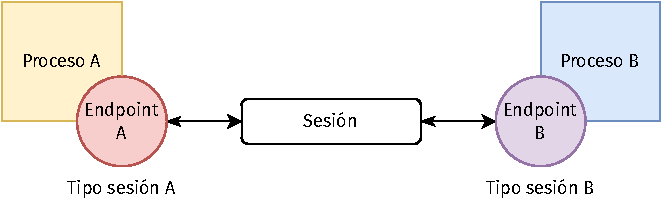
\includegraphics[width=0.8\textwidth]{images/tipo-sesion.pdf}
		\caption{Estructura de comunicación mediante tipos sesión}
	\end{figure}
\end{frame}

\subsection{Ejemplo: Describiendo suma con tipos sesión}

\begin{frame}{\insertsubsection}
	Consideremos un protocolo básico para la suma de dos números:
	\begin{enumerate}
		\item Cliente envía primer sumando
		\item Cliente envía segundo sumando
		\item Servidor retorna suma
	\end{enumerate}
\end{frame}

\begin{frame}{\insertsubsection}
	\begin{figure}
		\centering
		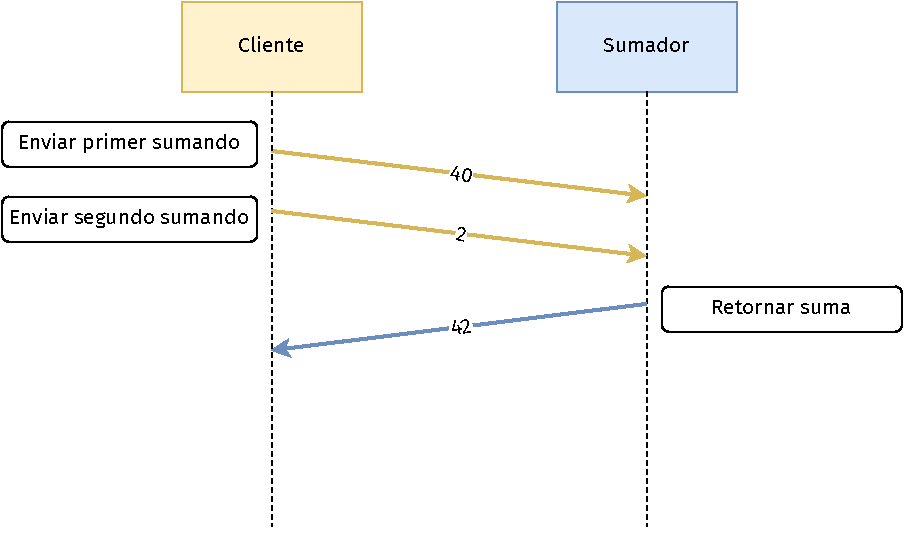
\includegraphics[width=0.9\textwidth]{images/sum-diagram.pdf}
		\caption{Ejemplo de comunicación para servicio sumador}
	\end{figure}
\end{frame}

\begin{frame}{\insertsubsection}
	\begin{figure}
		\centering
		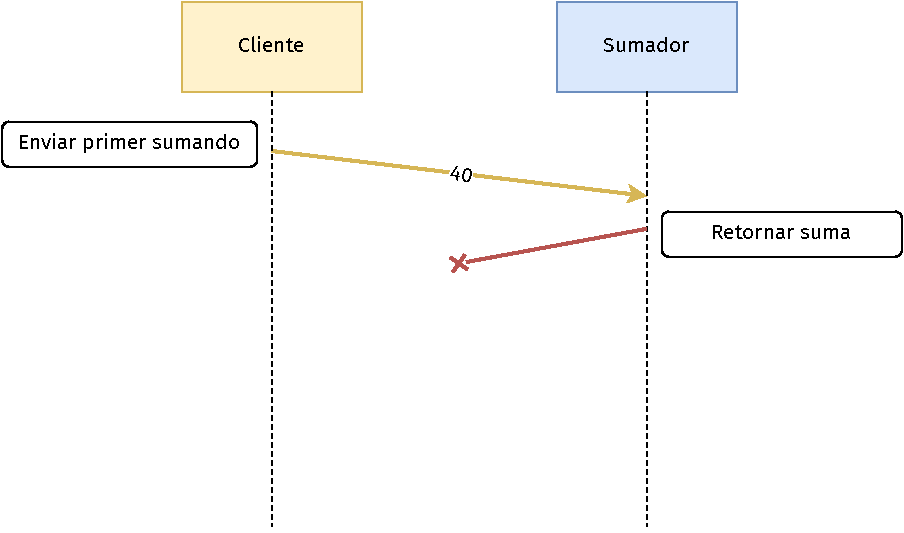
\includegraphics[width=0.9\textwidth]{images/sum-diagram-illegal.pdf}
		\caption{Violación de linearidad}
	\end{figure}
\end{frame}

\begin{frame}{\insertsubsection}
	\begin{figure}
		\centering
		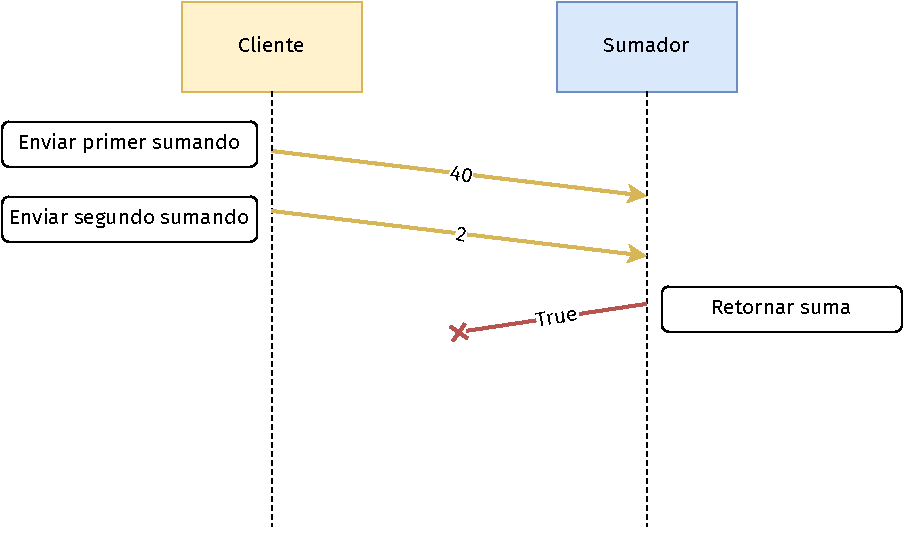
\includegraphics[width=0.9\textwidth]{images/sum-diagram-type-violation.pdf}
		\caption{Tipo de valor de retorno inválido}
	\end{figure}
\end{frame}

\begin{frame}{\insertsubsection}
	Para este ejemplo, la comunicación podría estructurarse mediante los siguientes tipos sesión:
	\begin{itemize}
		\item \textbf{Cliente:} $\SessionType = \Out\tint{ \Out\tint{ \In\tint\End } }$
		\item \textbf{Sumador:} $\dual\SessionType = \In\tint{ \In\tint{ \Out\tint\End } }$
	\end{itemize}

	\begin{figure}
		\centering
		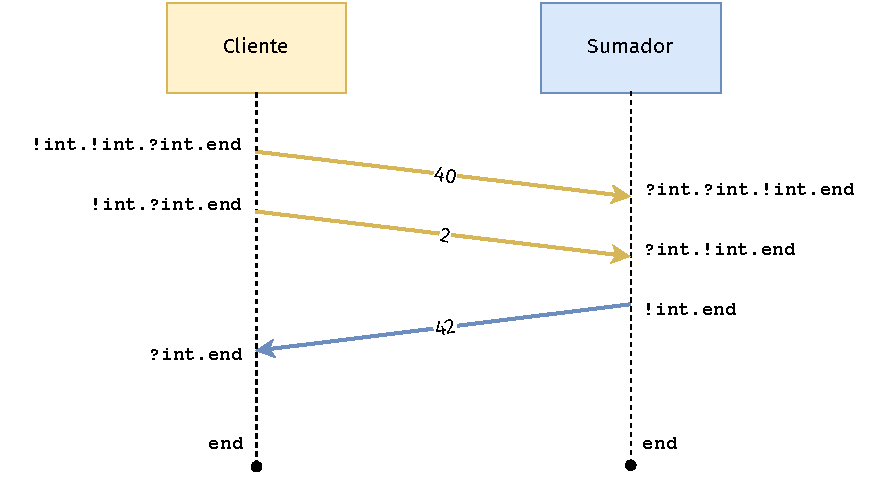
\includegraphics[width=0.9\textwidth]{images/sum-diagram-st.pdf}
	\end{figure}
\end{frame}

\subsection{Implementación de tipos sesión: FuSe}

\begin{frame}{\insertsubsection}
	\FuSe \footfullcite{DBLP:journals/jfp/Padovani17} es una biblioteca que habilita el uso de tipos sesión binarios en
	\OCaml.
	\begin{itemize}
		\item Codificación basada en igualdad de tipos y tipos parametrizados.
		\item Detección de violaciones de linearidad en tiempo de ejecución.
		\item Garantiza comunicación segura, fidelidad y progreso (siempre y cuando no haya deadlocks y se respete la linearidad).
		\item Inferencia de tipos y subtipado provisto por el sistema de tipos de \OCaml.
	\end{itemize}
	\begin{figure}
		\centering
		
\includegraphics[width=0.3\textwidth]{images/ocaml-logo.png}
	\end{figure}
\end{frame}

\begin{frame}{\insertsubsection}
	\SumClient
	Evolución del tipo sesión:
	\begin{itemize}
		\item \OI{ep0:} $\Out\tint{ \Out\tint{ \In\tint\End } }$
		\item \OI{ep1:} $\Out\tint{ \In\tint\End }$
		\item \OI{ep2:} $\In\tint\End$
		\item \OI{ep3:} $\End$
	\end{itemize}
\end{frame}

\begin{frame}{\insertsubsection}
	\SumServer
	Creamos un \emph{thread} con el sumador y realizamos una suma con el cliente:
	\SumExample
\end{frame}

\subsection{Elecciones}

\begin{frame}{\insertsubsection}
	Además de enviar y recibir, un protocolo puede presentar bifurcaciones,
	elecciones que impacten en cómo se desarrolla el mismo.

	\SumServerRec

	Donde \OI{ep0} es un endpoint de tipo sesión: $\SessionType = \In\tint{ \In\tint{
		\Out\tint\BinaryPBranch[]\T\End } }$
\end{frame}

\begin{frame}{\insertsubsection}
	\SumThreeNumClient
	Donde \OI{ep0} es un endpoint de tipo sesión: $\dual\SessionType = \Out\tint{ \Out\tint{
		\In\tint{\Choice\set{\Tag[True]: \Out\tint{ \Out\tint{
		\In\tint{\Choice\set{\Tag[False]: \End} }}}} }}}$
\end{frame}

\section{Tipos sesión probabilísticos}

\begin{frame}{\insertsection: Subasta}
	En \emph{``Probabilistic Analysis of Binary Sessions''}\footfullcite{DBLP:conf/concur/InversoMPTT20} se propuso el uso de tipos de sesión
	para razonar probabilísticamente sobre propiedades de alcanzabilidad,
	donde se dio una interpretación \emph{probabilística} a los operadores
	de selección.

	\begin{itemize}
		\item Salto de interpretación no determinística a una
		probabilística.
		\item Sistema de tipos que permite determinar la probabilidad con la que una
			sesión termina \emph{exitosamente}.
	\end{itemize}

	Existen protocolos donde la toma de elecciones con cierta probabilidad
	es requisito para cumplir las garantías del mismo (Ejemplo: seguridad, anonimato).
\end{frame}

%\begin{frame}{\insertsubsection: Motivación}
%
%	En el protocolo \textbf{Crowds}, el anonimato se logra \emph{escondiendo} al
%	usuario que inició la conversación mediante saltos aleatorios.
%
%	\begin{figure}
%		\centering
%		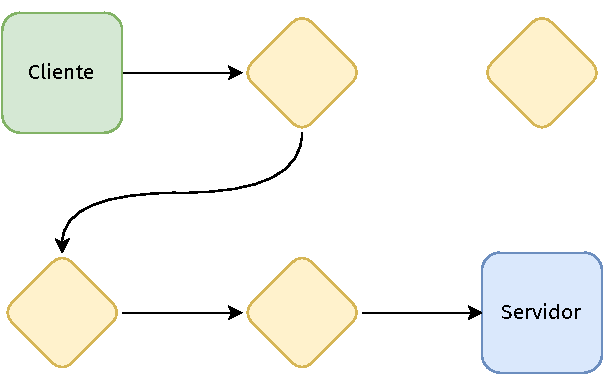
\includegraphics[width=0.5\textwidth]{images/crowds-protocol.pdf}
%	\end{figure}
%
%	\begin{itemize}
%		\item Una \emph{crowd} (multitud) de $N$ usuarios participa en el protocolo.
%		\item El cliente selecciona un usuario al azar.
%		\item Cada usuario selecciona probabilísticamente:
%		\begin{itemize}
%			\item Con probabilidad $p$ redirigir el mensaje a otro usuario.
%			\item Con probabilidad $1 - p$ enviar el mensaje al destino final (servidor).
%		\end{itemize}
%	\end{itemize}
%\end{frame}

\begin{frame}{\insertsection: Subasta}
	\begin{enumerate}
		\item Comprador envía oferta.
		\item Subastador:
			\begin{itemize}
				\item Vende artículo con probabilidad $\frac{1}{4}$
				\item Realiza contraoferta con probabilidad $\frac{3}{4}$.
			\end{itemize}
		\item Comprador (Si el artículo no se vendió):
			\begin{itemize}
				\item Vuelve a ofertar con probabilidad $\frac{1}{3}$.
				\item Abandona subasta con probabilidad $\frac{2}{3}$
			\end{itemize}
	\end{enumerate}
\end{frame}

\begin{frame}{\insertsection: Subasta}
	\begin{figure}
		\centering
		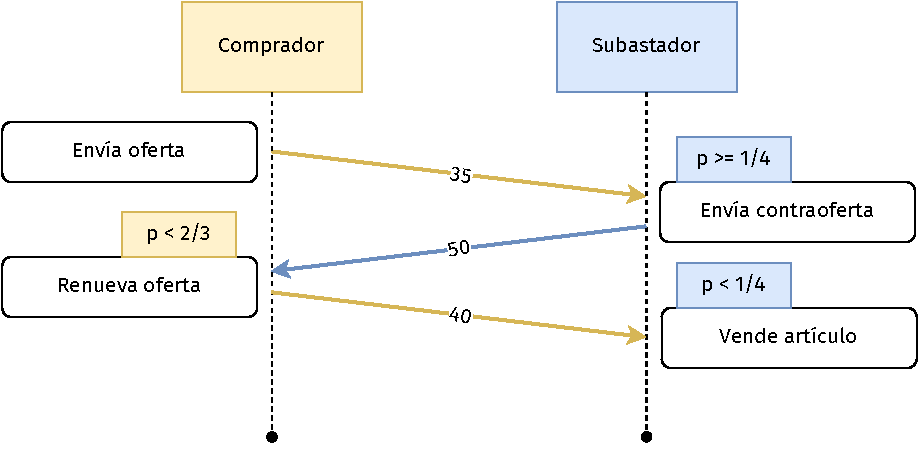
\includegraphics[width=0.9\textwidth]{images/auction-diagram.pdf}
		\caption{Ejemplo de subasta, $p \sim U(0, 1)$}
	\end{figure}
\end{frame}

\begin{frame}{\insertsection: Subasta}
	\AuctionBuyer[basicstyle=\footnotesize]
\end{frame}

\begin{frame}{\insertsection: Subasta}
	\Auctioneer[basicstyle=\footnotesize]
\end{frame}

\begin{frame}{\insertsection: Subasta}
	El tipo sesión que describe la interacción del Comprador es:
	\begin{equation*}
	    \label{eq:refined.auction}
	    \SessionType = \Out\tint{
		\BinaryPBranch[\frac{1}{4}]\Done{
		    \In\tint{
			\BinaryPChoice[\frac{2}{3}]\T\Idle
		    }
		}
	    }
	\end{equation*}

	Dado que no existe una interpretación universal de ``terminación
	exitosa'', se diferencia la terminación exitosa ($\Done$) de la
	infructuosa ($\Idle$) mediante constructores dedicados.

	\pause
	En este caso, la probabilidad de éxito (se concreta la venta) es de $\frac{1}{3}$.
\end{frame}

\section{Cambios a interfaz programática}

\begin{frame}[fragile]{\insertsection}

	\begin{table}[htb]
	    \begin{OCamlD}[basicstyle=\scriptsize,frame=single]
        val create  : unit -> $\etvar$ * $\sdual\etvar$
        val close   : $\End$ -> unit
        val send    : $\tvar$ -> $\Out\tvar\etvar$ -> $\etvar$
        val receive : $\In\tvar\etvar$ -> $\tvar$ * $\etvar$
        val select_true  : $\Choice\set{\Tag[True]: \etvarA}$ -> $\etvarA$
        val select_false : $\Choice\set{\Tag[False]: \etvarB}$ -> $\etvarB$
        val branch       : $\BinaryPBranch[]{\etvarA}{\etvarB}$ -> $\set{\Tag[True]: \etvarA,\ \Tag[False]: \etvarB}$
	    \end{OCamlD}
	\end{table}
\pause
	\begin{table}[htb]
	    \begin{OCamlD}[basicstyle=\scriptsize,frame=single]
        val create  : unit -> $\etvar$ * $\sdual\etvar$
        val close   : $\Done$ -> unit
        val idle    : $\Idle$ -> unit
        val send    : $\tvar$ -> $\Out\tvar\etvar$ -> $\etvar$
        val receive : $\In\tvar\etvar$ -> $\tvar$ * $\etvar$
        val select_true  : $\BinaryPChoice[1]{\etvarA}{\etvarB}$ -> $\etvarA$
        val select_false : $\BinaryPChoice[0]{\etvarA}{\etvarB}$ -> $\etvarB$
        val pick         : $p$ -> $(\BinaryPChoice[0]{\etvarA}{\etvarB}$ -> $\alpha)$
                             -> $(\BinaryPChoice[1]{\etvarA}{\etvarB}$ -> $\alpha)$
                             -> $\BinaryPChoice[p]{\etvarA}{\etvarB}$ -> $\alpha$
        val branch       : $\BinaryPBranch[p]{\etvarA}{\etvarB}$ -> $\set{\Tag[True]: \etvarA,\ \Tag[False]: \etvarB}$
	    \end{OCamlD}
	\end{table}
\end{frame}

\section{Elecciones probabilísticas}

\begin{frame}{\insertsection}
	En el cálculo de tipos sesión probabilísticos se utiliza el operador
	$\csum{}{}$ para definir la combinación de tipos en una elección probabilística:
	\begin{equation*}
	    \csum{t}{s}
	    \eqdef
	    \begin{cases}
	      t & \text{si $t = s$}
	      \\
	      \BinaryPChoice[pq+(1-p)r]{\SessionTypeT}{\SessionTypeS} & \text{si $t = \BinaryPChoice[q]{\SessionTypeT}{\SessionTypeS}$} \\ & \text{y $s = \BinaryPChoice[r]{\SessionTypeT}{\SessionTypeS}$}
	      \\
	      \text{indefinido} & \text{caso contrario}
	    \end{cases}
	\end{equation*}
	\pause
	En base a esto, el tipo de \OI{pick} debía cumplir con los siguientes requisitos:
	\begin{itemize}
		\item Seleccionar rama $\SessionTypeT$ con probabilidad $pq + (1 - p)r$.
		\item Seleccionar rama $\SessionTypeS$ con probabilidad $1 - (pq + (1 - p)r)$.
		\item Reflejar probabilidad $pq + (1 - p)r$ en la elección del tipo sesión.
		\item Permitir únicamente combinación de \emph{tipos compatibles}.
	\end{itemize}
\end{frame}

\begin{frame}[fragile]{\insertsection}
	\begin{table}[htb]
	    \begin{OCamlD}[basicstyle=\scriptsize,frame=single]
              val pick : $p$ -> $(\BinaryPChoice[0]{\etvarA}{\etvarB}$ -> $\alpha)$
                           -> $(\BinaryPChoice[1]{\etvarA}{\etvarB}$ -> $\alpha)$
                           -> $\BinaryPChoice[p]{\etvarA}{\etvarB}$ -> $\alpha$
	    \end{OCamlD}
	\end{table}
	\CoinFlipSumServer[basicstyle=\footnotesize]

	\begin{equation*}
		\SessionType = \BinaryPChoice[\frac{1}{2}]{
			\In\tint{\In\tint{\Out\tint{\Done}}}
			}{\Idle}
	\end{equation*}
\end{frame}

\subsection{Elecciones multi-sesión}

\begin{frame}{\insertsubsection}
	Hasta ahora trabajamos con protocolos que interactúan solamente con una sesión.
	\pause
	\InvalidCoinFlipSumServer[basicstyle=\footnotesize]
\end{frame}

\begin{frame}{\insertsubsection}
	
	En el cálculo probabilístico, la regla \rulename{t-choice} (debajo
	adaptada a nuestra extensión) combina probabilísticamente los contextos
	de tipado de cada rama de una elección:
	\begin{gather*}
	\inferrule[\rulename{t-choice}]{
	  \wtp \EmptyContext prob : p
	  \\
	  \wtp\ContextA P : \sigma
	  \\
	  \wtp\ContextB Q : \sigma
	}{
		\wtp{\csum\ContextA\ContextB}{\text{\OI{pick}} \ prob \ P \ Q} : \sigma
	}
	\end{gather*}
	\pause
	Nuestra primitiva \OI{pick} no recibe ninguna información de tipo de \OI{epY}.

	Se suman así las siguientes restricciones:
	\begin{itemize}
		\item Capturar a nivel de tipo sesiones adicionales.
		\item Forzar el uso de formas compatibles.
	\end{itemize}
\end{frame}

\begin{frame}[fragile]{\insertsubsection}
	\begin{OCamlD}[basicstyle=\scriptsize,frame=single]
	val pick_2ch:
	    $p$ -> $(\BinaryPChoice[0]{\etvarA}{\etvarB}$ -> $\BinaryPChoice[r]{\etvarC}{\etvarD}$ -> $\alpha)$
	      -> $(\BinaryPChoice[1]{\etvarA}{\etvarB}$ -> $\BinaryPChoice[q]{\etvarC}{\etvarD}$ -> $\alpha)$
	      -> $\BinaryPChoice[p]{\etvarA}{\etvarB}$ -> $\BinaryPChoice[pq + (1 - p)r]{\etvarC}{\etvarD}$
	      -> $\alpha$
	\end{OCamlD}
	\pause
	\ValidCoinFlipSumServer[basicstyle=\footnotesize]
\end{frame}

\section{Composición de tipos sesión duales}

\begin{frame}{\insertsection}
	La creación de una sesión devuelve un par de tipos
	sesión duales $\SessionType$ y $\dual\SessionType$.
	
	Su composición al momento de estructurar una comunicación brinda la
	información necesaria para calcular la probabilidad de éxito en el tipo
	\alert{$\ClosedSessionType$}.

	\pause
	Elegir una representación adecuada para este tipo presenta algunos desafíos.
	\begin{itemize}
		\item Para el cálculo de éxito, debe capturar la información de
			tipo de sus endpoints ($\SessionType$ o su dual
			$\dual\SessionType$).
		\item Se encuentra sujeta a la combinación probabilística vista anteriormente.
	\end{itemize}
\end{frame}

\begin{frame}[fragile]{\insertsection}
	Nuestra representación toma la forma de un argumento opcional (\OI{?st}) en la primitiva
	\OI{create}.

	Al ser un tipo informativo, el uso de un argumento opcional permite
	ignorarlo y aún así disponer de las garantías de tipo que provee
	nuestra extensión.
	\begin{OCamlD}[basicstyle=\scriptsize,frame=single]
              type $\etvar$ cpst
              val create  : ?st:$\etvar$ cpst -> unit -> $\etvar$ * $\sdual\etvar$
              val cst_placeholder : $\etvar$ cpst
	\end{OCamlD}
	Como sólo nos interesa el tipo de nuestro argumento
	opcional, definimos la constante \OI{cst_placeholder} que tipa como una
	sesión cerrada para utilizar como valor por defecto.
\end{frame}

\begin{frame}[fragile]{\insertsection}
	\TestBuyerAuctioneer[basicstyle=\footnotesize]
	Posterior al cálculo de probabilidad de éxito, el tipo de la función es:
	\begin{OCamlD}[basicstyle=\footnotesize,frame=single]
    val test_buyer_auctioneer  : ?st:$\ClosedSessionType[\frac{1}{3}]$ -> unit -> unit
	\end{OCamlD}
\end{frame}

%\subsection{Combinación multi-sesión}
%
%\begin{frame}{\insertsubsection}
%	Contar cómo se repite el mismo problema que con las elecciones multisesión
%\end{frame}
%
%\begin{frame}{\insertsubsection}
%	Mencionar caminos posibles y solución utilizada
%\end{frame}

\section{Codificación de probabilidades}
\begin{frame}[fragile]{\insertsection}
	La representación de las probabilidades es esencial para el posterior
	cálculo de probabilidad de éxito.
	
	\pause Definimos $p$ como la probabilidad con la que se envía
	($\BinaryPChoice{\etvarA}{\etvarB}$) o recibe
	($\BinaryPBranch{\etvarA}{\etvarB}$) la elección de seguir por
	$\Tag[True]$.

	Normalmente podría utilizarse una representación de coma flotante como
	\OI{float}, el problema con tal modelo es que no brinda información del
	valor de $p$ en tiempo de compilación:

	\begin{OCamlD}[basicstyle=\footnotesize,frame=single]
  let p = 0.75;; (* definimos constante con valor 0.75 *)
  val p : float  (* tipo de dato obtenido *)
	\end{OCamlD}
\end{frame}

\subsection{Representando naturales}
\begin{frame}[fragile]{\insertsubsection}

	\begin{OCamlD}[basicstyle=\footnotesize,frame=single]
  type _z
  type _s
  type _ nat = Z : _z nat | S : 'a nat -> (_s * 'a) nat
	\end{OCamlD}
	\begin{itemize}
		\item Definimos los tipos \OI{_z} y \OI{_s} como etiquetas
			para distinguir a nivel tipo entre cero y la función
			sucesor.
		\item Definimos \OI{nat} como una estructura de datos
			algebraica particular denominada GADT (Generalized
			Algebraic Data Type) que permite establecer
			restricciones en los parámetros de sus constructores.
	\end{itemize}

	\pause
	Construcción de primeros naturales y el cero:
		\begin{OCamlD}[basicstyle=\footnotesize,frame=single]
  let zero : _z nat = Z
  let one : (_s * _z) nat = S Z
  let two : (_s * (_s * _z)) nat = S (S Z)
		\end{OCamlD}
\end{frame}

\subsection{Representando racionales}
\begin{frame}[fragile]{\insertsubsection}
	\begin{OCamlD}[basicstyle=\footnotesize,frame=single]
    type _ frac = Fraction : 'a nat * (_s * 'b) nat ->
                            ('a nat * (_s * 'b) nat) frac
	\end{OCamlD}


	\begin{itemize}
		\item Definimos \OI{frac} como otro GADT que permite la
			construcción de números racionales.
		\item El mismo toma tupla cuya primer componente representa al
			numerador y la segunda el denominador, prohibiendo el
			cero mediante una restricción de tipo.
	\end{itemize}

	\pause
	A modo de ejemplo damos la construcción para $\frac{1}{2}$:
	\begin{OCamlD}[basicstyle=\footnotesize,frame=single]
    let one_half : ((_s * _z) nat *
                    (_s * (_s * _z)) nat) frac
                    = Fraction (S Z, S (S Z))
	\end{OCamlD}
\end{frame}

\section{Probabilidad de éxito de una sesión}
\begin{frame}{\insertsection}

		La \emph{probabilidad de éxito} de un tipo sesión $\SessionType$,
		denotada como $\psfun\SessionType$, se encuentra definida por
		las siguientes ecuaciones:
	  \[
	    \begin{array}{r@{~}c@{~}l}
	      \psfun\Idle & = & 0 \\
	      \psfun\Done & = & 1 \\ 
	    \end{array}
	    \quad
	    \begin{array}{r@{~}c@{~}l}
	      \psfun{\In\Type\SessionType} & = & \psfun\SessionType \\
	      \psfun{\Out\Type\SessionType} & = & \psfun\SessionType \\
	    \end{array}
	  \]
	\[
	    \begin{array}{r@{~}c@{~}l}
	      \psfun{\BinaryPBranch\SessionTypeT\SessionTypeS} & = & p\psfun\SessionTypeT + (1-p)\psfun\SessionTypeS \\
	      \psfun{\BinaryPChoice\SessionTypeT\SessionTypeS} & = & p\psfun\SessionTypeT + (1-p)\psfun\SessionTypeS \\
	    \end{array}
	\]

	Para un tipo sesión $\SessionType$ \emph{finito}, la definición describe un
	algoritmo recursivo para el cómputo de $\psfun\SessionType$.
\end{frame}

\begin{frame}{\insertsection}
	Cuando $\SessionType$ es infinito (un protocolo recursivo), puede
	interpretarse como una Cadena de Markov en Tiempo
	Discreto\footnote{Discrete-Time Markov Chain, DTMC)} cuyo espacio de
	estados es $\trees\SessionType = \mathset{S_1, \dots, S_n}$ y tal que
	la probabilidad $p_{ij}$ de transicionar de un estado $S_i$ al estado
	$S_j$ está dada por
	\[
  p_{ij} \eqdef
  \begin{cases}
    p & \text{si $S_i \tred[p] S_j$}
    \\
    0 & \text{caso contrario}
  \end{cases}
	\]

	\begin{itemize}
		\item Siempre es posible alcanzar un \emph{estado absorbente}
			($\Done$ ó $\Idle$) desde cualquier \emph{estado
			transitorio} (cualquier otro tipo sesión).
		\item La probabilidad de alcanzar un estado absorbente desde
			uno transitorio puede ser computado mediante la
			resolución de un sistema de ecuaciones para el cual se
			garantiza
			una solución única~\footfullcite{KemenySnell}.
	\end{itemize}
\end{frame}

\subsection{Extendiendo decodificación de tipos sesión: rosetta}
\begin{frame}[fragile]{\insertsubsection}

	\texttt{rosetta} es la herramienta que acompaña \FuSe para decodificar
	los tipos generados por \OCaml.

	\begin{table}[htb]
		\begin{OCamlD}[basicstyle=\footnotesize,frame=single]
  val send    : 'a -> (_0,('a * ('s,'r) pst)) pst -> ('r,'s) pst
  val receive : (('a * ('r,'s) pst),_0) pst -> 'a * ('r,'s) pst
		\end{OCamlD}
		\caption{Ejemplo de tipos sin decodificar.}
	\end{table}

	\pause
	La extensión al cálculo de tipos sesión probabilísticos consistió de dos
	partes:
	\begin{itemize}
		\item Modificar la función decodificadora para considerar tipos
			probabilísticos y constructores de terminación exitosa.
		\item Calcular la probabilidad de éxito para tipos sesión
			cerrados $\ClosedSessionType$.
	\end{itemize}
\end{frame}

\section{Conclusión y trabajo a futuro}
\begin{frame}{\insertsection}
	Aportes de este trabajo:
	\begin{itemize}
		\item Contribución a popularización y uso de tipos comportamentales como los
			tipos sesión.
		\item Extensión que implementa el cálculo de tipos sesión
			probabilísticos sin perder las garantías del sistema
			original (\FuSe).
		\item Representación e inferencia de tipos sesión
			probabilísticos con una interfaz programática enfocada
			en la usabilidad del sistema.
		\item Implementación libre de funcionalidades avanzadas del
			lenguaje de como lo pueden ser el uso de mónadas o
			sistemas de tipo sub-estructurales.
	\end{itemize}
\end{frame}

\begin{frame}{\insertsection}
	Trabajo a futuro:
	\begin{itemize}
		\item Implementación de distribuciones de probabilidad para
			tratar elecciones con más de una rama.
		\item Extensión al decodificador de tipos para que utilice
			alguna representación simbólica para variables libres y
			retorne un resultado en función de las mismas.
	\end{itemize}
\end{frame}

\begin{frame}{Fin}
	\begin{center}
	\Huge ¡Muchas gracias!

	\bigskip

	\Huge ¿Preguntas?
	\end{center}
\end{frame}
